\documentclass[12pt]{article}
\usepackage{etoolbox}
\usepackage{float}
\usepackage{graphicx}
\usepackage[justification=centering]{caption}

\makeatletter
\patchcmd{\l@section}
{\hfil}
{\leaders\hbox{\normalfont$\m@th\mkern \@dotsep mu\hbox{.}\mkern \@dotsep mu$}\hfill}
{}{}
\makeatother
\begin{document}
	
	\begin{titlepage}
		
		\newcommand{\HRule}{\rule{\linewidth}{0.5mm}} % Defines a new command for the horizontal lines, change thickness here
		
		\center % Center everything on the page
		
		%----------------------------------------------------------------------------------------
		%	HEADING SECTIONS
		%----------------------------------------------------------------------------------------
		
		\textsc{\LARGE Illinois Institute of Technology}\\[1.5cm] % Name of your university/college
	%	\textsc{\Large Major Heading}\\[0.5cm] % Major heading such as course name
		%\textsc{\large Minor Heading}\\[0.5cm] % Minor heading such as course title
		
		%----------------------------------------------------------------------------------------
		%	TITLE SECTION
		%----------------------------------------------------------------------------------------
		
		\HRule \\[0.4cm]
		{ \huge \bfseries ECE 441 Monitor Project}\\[0.4cm] % Title of your document
		\HRule \\[1.5cm]
		
		%----------------------------------------------------------------------------------------
		%	AUTHOR SECTION
		%----------------------------------------------------------------------------------------
		
		\begin{minipage}{0.4\textwidth}
			\begin{flushleft} \large
				\emph{Author:}\\
				Adam \textsc{Sumner} % Your name
			\end{flushleft}
		\end{minipage}
		~
		\begin{minipage}{0.4\textwidth}
			\begin{flushright} \large
				\emph{Teaching Assistant:} \\
				Boyang \textsc{Wang} % Supervisor's Name
			\end{flushright}
		\end{minipage}\\[4cm]
		
		% If you don't want a supervisor, uncomment the two lines below and remove the section above
		%\Large \emph{Author:}\\
		%John \textsc{Smith}\\[3cm] % Your name
		
		%----------------------------------------------------------------------------------------
		%	DATE SECTION
		%----------------------------------------------------------------------------------------
		
		{\large April 28th, 2015}\\[3cm] % Date, change the \today to a set date if you want to be precise
		
		%----------------------------------------------------------------------------------------
		%	LOGO SECTION
		%----------------------------------------------------------------------------------------
		
		%\includegraphics{Logo}\\[1cm] % Include a department/university logo - this will require the graphicx package
		
		%----------------------------------------------------------------------------------------
		
		\vfill % Fill the rest of the page with whitespace
		
		\textbf{Acknowledgment} \\ \flushleft I acknowledge all of the work including figures and code belongs to me and/or persons who are referenced.
	\end{titlepage}
	
	\tableofcontents
	\newpage
	\addtocontents{toc}{~\hfill\textbf{Page}\par}
	%\chapter{...}
	\begin{abstract}
		This project involved designing and implementing a Monitor program using the MC68000 assembly language. The program implements twelve basic debugger functions as well as two author defined functions. It is designed to handle exceptions, and is meant to be an educational piece of software for students taking ECE 4411 at the Illinois Institute of Technology.
	\end{abstract}
	
	\section{Introduction}
	The \textsc{Sanper-1 ELU} is a Motorola MC68000 based microcomputer designed by Dr. Jafar Saniie and Mr. Stephen Perich for use in college level computer engineering courses. For user interaction, it utilizes a monitor program called TUTOR that enables users to actively interact with the microcomputer. The design objective of this project is to re-implement the functionality of TUTOR into a student written monitor program titled MONITOR441. The program should be able to perform basic debugger functions such as memory display, memory sort, memory change, etc., and must have the ability to handle exceptions. The design constraints are:
	\begin{itemize}
		\item Code must be smaller that 3K starting from address \$1000
		\item Stack size must be 1K starting at memory location \$3000
		\item Macros may not be used
		\item Erroneous inputs should not kill the program
	\end{itemize}
	Twelve debugger functions must be implemented, along with two user defined debugger commands.
	
	\section{Monitor Program}
	The monitor program operates in a command driven environment. It acts as a typical shell, providing a user interface to access the microcomputer's services. The main program being run is a command line interpreter. Based on the input that the user enters, the interpreter determines if the input entered is valid and subsequently executes the specified command. The structure of how this program operates is shown in Figure \ref{fig:monitor}.
		\begin{figure}[H]
			\centering
			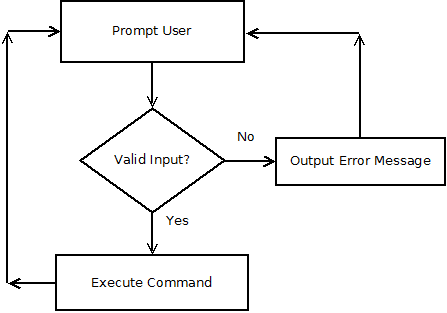
\includegraphics[width=0.7\linewidth]{monitor.png}
			\caption{Structure of Monitor Program}
			\label{fig:monitor}
		\end{figure}
		
		\subsection{Command Interpreter}
			\subsubsection{Algorithm and Flowchart}
			The algorithm for the command interpreter uses simple string matching to determine if input is correct. The algorithm begins by outputting the message \texttt{MONITOR441>} and accepting input from the user. It then checks for the ASCII value \$48 which corresponds to the letter H. This is to check for either the \texttt{HELP} command or \texttt{HXDC} command. If an H was not entered, it then checks for the ASCII value \$4D which corresponds to a memory command. If this fails, then it checks for ASCII value \$47, corresponding to the \texttt{GO} command. If this fails, the ASCII value \$44 is tested, corresponding to the \texttt{DF} command. If this fails, it checks for \$42, which signifies a \texttt{BLCK} command. If this fails, \$53 is tested for the \texttt{SORTW} command. If this fails, \$45 is tested for the \texttt{ECHO} command. If this fails \$2E is checked for the modify register command. If all of these checks fail, the user has entered incorrect input and an error message is displayed. If any of these checks succeed, the command line interpreter jumps to the respective command's helper interpreter function. These subroutines check for each character of the user input in order to verify the command the user entered was correct. These helper functions also serve to differentiate commands that start with the same character. The flowchart for this process is shown in Figure 
			\subsubsection{68000 Assembly Code}
\end{document}